\chapter{Metodología}

\textbf{Buscamos describir cómo abordamos el desarrollo del problema y su solución}.
Leyendo este capítulo el lector conocerá la metodología que empleamos al desarrollar este
proyecto.

Es inmensamente doloroso el poco tiempo que vivimos, pero es que es más doloroso dedicar
nuestro tiempo a tareas que no benefician a aquellos entes a los cuales queremos aportar
valor.
A lo largo de este Trabajo de Fin de Grado exponemos diversos métodos para minimizar
el tiempo invertido en tareas sin valor \textbf{para nuestro propósito}.\footnote{%
    No es lo mismo pilotar un avión tetrarreactor Airbus A380,
    un avión de negocios Gulfstream G800 que una avioneta Cessna 172.
}

Nos servimos de distintos métodos para descubrir, esclarecer y categorizar el conocimiento que necesitamos
para desarrollar un sistema informático: correcta identificación del problema a resolver,
mejor solución posible teniendo en cuenta el entorno en el que se utilizará,
y formulación de la solución de este en términos de datos objetivos acerca de cómo debe de
funcionar un sistema.

\section{Cuestiones previas}

Exponemos información complementaria a las ideas de las secciones de este capítulo.

\subsection{Definiciones}

Utilizamos determinadas acepciones definidas por \cite{RAE_DLE}.

Entendemos el \textbf{arte} como la ``capacidad, habilidad para hacer algo'' y como
el ``conjunto de preceptos y reglas necesarios para hacer algo''.

Entendemos por \textbf{técnica} como aquello ``perteneciente o relativo a las
aplicaciones de las ciencias y de las artes''.

Entendemos por \textbf{método} como ``procedimiento que se sigue en las ciencias
para hallar la verdad y enseñarla.''

Entendemos por \textbf{metodología} el ``conjunto de métodos que se siguen en una investigación
científica o en una exposición doctrinal''.

Entendemos por \textbf{tecnología} como el ``conjunto de teorías y de técnicas que permiten el
aprovechamiento práctico del conocimiento científico''.

Entendemos por \textbf{herramienta} como un ``instrumento que sirve para hacer algo o
conseguir un fin''.

\subsection{La importancia del método}

Los cirujanos, sujetos cognoscentes, operan mediante su cuerpo y herramientas a los seres
vivos para curar, restablecer, aliviar, mejorar o embellecer partes de un cuerpo de
un ser vivo. En este proceso utilizan su conocimiento de las tecnologías pertinentes.
De una forma ordenada y deliberada realizan el procedimiento que consideran adecuado para
lograr su objetivo.

Cuando investigan buscan esclarecer la realidad que se les presenta. Descubren, aclaran y
categorizan.

Según el Diccionario panhispánico del español jurídico, a la ingeniería se la define
de forma general como sigue.

\begin{quote}
    \textit{
    ``Conjunto de conocimientos y técnicas científicas y empíricas aplicadas a la invención,
    el diseño, el desarrollo, la construcción, el mantenimiento y el perfeccionamiento
    de tecnologías, estructuras, máquinas, herramientas, sistemas, materiales y procesos
    para la resolución de problemas prácticos''.
    }
\end{quote}

Sabemos empíricamente que nuestra capacidad para lidiar con la complejidad de forma exacta
es limitada. Además, nuestros procesos, influenciados por el conocimiento que almacenamos (y que recuperamos
principalmente cuando se da un determinado contexto que \textit{activa} este conocimiento),
\textit{siguen un único hilo racional}. Sabemos que \textbf{dadas unas premisas}, existen \textbf{técnicas
no rigurosas} que suelen ser efectivas a la hora de buscar soluciones. Conocemos qué caracteriza
a aquellos proyectos correctos, funcionales, profesionales y de calidad.

Un método por sí solo no tiene capacidad para operar la realidad. Pero nosotros podemos hacerlo.
Mediante nuestro criterio, moldeado por nuestra experiencia, seleccionamos qué queremos trabajar,
y cómo lo haremos\cite[Distinción entre método y metodología]{MetodoUNAM}.\footnote{%
Partiendo de esta definición y de las ideas de Bueno \cite{TeoríaDelCierreCategorial} exponemos
la siguiente tesis.
Un ingeniero opera la realidad con un propósito utilitario. No casualmente sino deliberadamente.
Lo hace por medio de \textit{``[...] tecnologías, estructuras, máquinas, [...]''}.
Por medio de materia y forma opera la realidad. Y operando la realidad modifica la materia y
la forma. De forma deliberada toma decisiones para su propósito. Maximiza la
efectividad de su solución para su propósito dados sus recursos materiales y de forma.
Busca mejorar la forma.
}
 Seguir un buen método para unas determinadas circunstancias nos puede permitir maximizar la
calidad de un producto. Su estructura y atomicidad potencia nuestras capacidades intelectuales
(lo que en el anterior párrafo podría verse como una limitación).
Gracias a que desglosa todas aquellas tareas y productos que podrían interesar desarrollar
en un producto de calidad es más difícil que se nos olviden, más cuando tenemos poca experiencia
o no tenemos todo memorizado.

\subsection{Ágil no es sinónimo de incompletud}

Existen empresas e individuales que se dedican a vender información y formación a otras empresas
o individuales. Es el caso de Robert C. Martin con su empresa Clean Coders, LLC. El caso de 
Ken Schwaber con scrum.org. Es el caso de Kent Beck con sus conferencias y libros. Es el caso
de Andy Hunt y Dave Thomas, \textit{los programadores pragmáticos}.

Estas y otras personas, las cuales se promulgan \textit{líderes} en sus respectivas metodologías,
se reúnen en febrero de 2001 en un resort de ski para encontrar un nexo en común
de sus acercamientos a la hora de desarrollar sistemas informáticos. Según se explica, este evento
se empieza a cocinar en una quedada de defensores del \textit{Extreme Programming}.
\textbf{Y agrupa a aquellos representantes de metodologías que en un principio 
Martin bautiza como \textit{ligeras}}.
\cite{HistoriaManifiestoAgilJim} \cite[Snowbird]{AgileBackToBasics}

El manifiesto ágil \cite{ManifiestoAgil} surge de este encuentro. Expone las siguientes ideas.

\begin{quote}
    \itshape{
    ``We are uncovering better ways of developing
    software by doing it and helping others do it.
    Through this work we have come to value:
    
    \textbf{Individuals and interactions} over processes and tools.

    \textbf{Working software} over comprehensive documentation.

    \textbf{Customer collaboration} over contract negotiation.

    \textbf{Responding to change} over following a plan.
    
    That is, while there is value in the items on
    the right, we value the items on the left more.''
    }
\end{quote}

Según documentan las fuentes, firmantes del manifiesto ágil \cite{ManifiestoAgil}, 
escriben el texto como contraposición a lo que observan en ciertas compañías a la
hora de desarrollar software. Dicen, rehúsan de los procedimientos sin sentido,
a los procedimientos sin un por qué. Alertan de que definitivamente dejarán de ser
compatibles con la incipiente modernización del mercado (expansión del comercio en
línea, compañías en línea, compañías web, etc). \cite{HistoriaManifiestoAgilJim}

Dicen que llegan a estas conclusiones a partir de su experiencia \cite{HistoriaManifiestoAgilJim}
y personalmente añadiría, \textit{y teniendo como objetivo la calidad del producto}.

El manifiesto es vago y no es exhaustivo, pero en ningún lugar se habla de no utilizar
procesos o herramientas.
No se desprestigia a la documentación. No se le resta valor a la negociación
de un contrato. No busca no seguir un plan.

\section{Uso de un repositorio}

Entendemos un repositorio como un lugar en el que almacenamos información.
En nuestro caso, información digital. Principalmente documentación, recursos
gráficos y código.

Utilizamos un único repositorio para facilitar el asegurar la coherencia
de los datos, mejorar la cohesión y organización de estos y facilitar su
recuperación.

En el repositorio únicamente almacenamos estados correctos del proyecto. No
almacenamos información que no sea relevante, como las que generan automáticamente
algunas herramientas. Siempre reflexionamos antes de realizar \textit{vendoring}%
\footnote{\textit{Vendoring} consiste en hacer copias de software de terceros en
nuestro propio repositorio. Por ejemplo, no suele tener sentido para una dependencia en
un paquete de \texttt{npm}. Se suele evitar hacer esto porque los software de control
de versiones para software no se suelen llevar bien con los binarios y porque que el código será
más difícil de actualizar.}.

\subsection{Seguimiento de cambios sobre el repositorio}

Sabemos que si a cada modificación que hacemos en el repositorio anotamos
lo que ha cambiado y por qué lo hemos hecho entonces tenemos distintas ventajas.

\begin{enumerate}
    \item Sabiendo la razón por la que se realiza un cambio ayudamos a entender
          el cambio a un tercero, o a nuestro yo del futuro.
    \item Podemos visitar estados anteriores del proyecto.
    \item Cuando liberamos una versión podemos saber qué ha cambiado desde la última
          versión, pudiendo ofrecer al cliente un histórico de cambios.
\end{enumerate}

Por convención los mensajes que acompañarán a estas \textit{contribuciones} vienen
dados en imperativo y serán claros y concisos, tal y como se propone en \cite[Commit Guidelines]{ProGIT}.

Si además estos cambios son para modificar un único aspecto del repositorio
entonces, además de potenciar los beneficios anteriores, tenemos las siguientes
ventajas entre otras.

\begin{enumerate}
    \item Deshacer cambios es más fácil.
    \item Identificar cambios concretos es más fácil. Por ejemplo, encontrar cuándo se introduce un bug
           es más fácil.
    \item El proceso de fusionar dos repositorios divergentes puede ser mas fácil y cómodo.
    \item La revisión por parte de un tercero, o por nosotros mismos, es mas clara.
    \item Es más fácil encontrar un mensaje descriptivo y conciso que explique qué cambia y por qué.
    \item Nos obliga a trabajar sobre un único aspecto del repositorio, lo que potencia nuestras
          capacidades intelectuales.
\end{enumerate}

Imponemos sendas restricciones en nuestro repositorio.

\subsection{Validez de los datos}

¿Qué determina la validez del repositorio? Su capacidad de despliegue en cualquier
momento de acuerdo a los requisitos que forman parte de los productos que componen
el repositorio.

No contribuimos en aquellos casos en los que no tenemos la certeza anterior.
Automatizamos en aquellos casos en los que estimemos que sea rentable en tiempo
y dinero.

\subsection{Uso de versionado semántico}

Los cambios sobre el repositorio siguen un orden cronológico.
Si un determinado cambio es el último que se hace antes de
liberar los productos que contienen el repositorio (por ejemplo,
cuando alcanzamos un hito) entonces a este cambio le asignamos
un nombre específico.

El nombre que le asignamos tiene que tener la forma \texttt{v[VERSION]},
donde \textit{\texttt{[VERSION]}} tiene la forma \texttt{[MAJOR].[MINOR].[PATCH]} y donde
\textit{\texttt{[MAYOR]}}, \textit{\texttt{[MINOR]}} y \textit{\texttt{[PATCH]}} son números que se
especifican según el esquema de versionado \textit{SemVer 2.0.0} \cite{SemVer}.
Escogemos este esquema de versionado porque es sencillo, bien conocido y se puede
entender de forma intuitiva.

\section{Indagación y esclarecimiento del problema a resolver}

Dialogamos con el cliente, formulamos el problema haciendo uso de las fases de
empatizar y definir del método \textit{Design Thinking} para después, tanto en un análisis
previo como a medida que vamos desarrollando el proyecto, extraer historias de usuario, historias de
desarrollador y \textit{user journeys} de donde obtenemos los objetivos deseados
junto a sus respectivas importancias.
Finalmente sintetizamos esta información en forma de requisitos funcionales y
requisitos no funcionales.

\subsection{Conversaciones con el cliente}

Este primer método lo ideamos una vez el cliente nos comunica brevemente su necesidad.
\textbf{Su principal objetivo es el de recuperar y modelar el problema a resolver}, ya sea en
el análisis previo o como complementario del análisis continuo, pero también busca
otros objetivos como el de transmitir confianza al cliente o el de ayudarnos como empresa a
decidir si esta será una batalla en la que nos gustaría e interesaría participar.

\textbf{El primer paso es que el cliente comunique su necesidad.} Sólo por el hecho de que esta
persona física o jurídica está depositando confianza en nosotros merece el más
adecuado respeto, que se demuestra dejándole el espacio que necesita para exponer
sus ideas. De esta descripción extraemos información verbal y
no verbal que nos ayuda a comprender las circunstancias en que ocurre el potencial
problema a resolver, y en caso de no ser un cliente de confianza o desconocer las
circunstancias en que se desenvuelve el problema, si como empresa nos interesa
ser un proveedor de soluciones para él y su sector.

De una forma atenta \textbf{y crítica} escuchamos y anotamos la información que el
cliente quiere transmitirnos. Si existe algún término que enuncia y desconocemos
o alguna circunstancia que nos describe y que no llegamos a comprender o bien le
interrumpimos o bien anotamos para preguntar más adelante.

\textbf{El segundo paso es identificar la raíz del problema.} Por experiencia sabemos
que las personas tienden a enunciar los problemas en términos de la solución.
Muchas veces aquello que nos solicitan responde a una necesidad subyacente que no
se identifica o, si identificada, no se comunica.

Buscamos dialogando con el cliente y por medio de nuestra propia investigación exponer
el problema eliminando las restricciones innecesarias, buscando aquellas que son
necesarias y, a poder ser, sin omitir aspectos que pudiesen afectar a la arquitectura
de la solución.

Por ejemplo, proponemos borradores rápidos de arquitectura los cuales
nuestro cliente puede analizar de forma crítica, de forma independiente
o por medio del método dialéctico. El interesado desmiente aquellos aspectos
pertinentes y saca a la luz nuevas necesidades y restricciones que no se habían
comunicado.

\textbf{El último paso consiste en formalizar las conversaciones} por medio de las
herramientas que estimemos según las circunstancias\footnote{%
    No utilizaremos las mismas herramientas y documentos para un cliente para el cual
    sabemos por experiencia qué es lo que quiere que para otro que nos exige resolver
    un problema de un sector y aplicación que desconocemos. También variamos según
    la capacitación técnica del cliente en nuestro dominio.
}. De esta forma, por medio de comunicaciones escritas, resolvemos el problema de
sincronizarnos con el cliente.

Por ejemplo, para los productos que desarrollamos en nuestro TFG, sabemos por experiencia
que para nuestros clientes y dado nuestro conocimiento en el sector el punto dulce está
en hacer un único documento en el que describimos hitos a alcanzar en el desarrollo.
Estos hitos los desglosamos en descripciones claras y concisas acerca del comportamiento del software.
A este documento lo llamamos \textbf{Plan de Desarrollo}.

Gracias a este documento el cliente puede darse
cuenta rápidamente de que estamos dedicando tiempo de desarrollo a un aspecto que no le
interesa desarrollar ahora mismo. Porque puede conocer en todo momento el estado del desarrollo.

\subsection{Contexto en el que se desarrolla el problema}

Para poder cuantificar de una aproximada el potencial de proyecto y para, en caso de que el
proyecto nos interese, formular los requisitos desde el punto de vista de los clientes que
interactuarán con nuestro producto, investigamos acerca del contexto que rodea al problema.

Descubrimos quiénes son los usuarios objetivo de nuestros productos y en qué contexto
interactuarían con el sistema.

\subsection{Investigación de los últimos avances (\textit{state-of-the-art})}

Investigamos si existen o no soluciones existentes para el problema. Si las existen,
las evaluamos y estudiamos su enfoque.

\section{Definición del problema a resolver (definición de requisitos)}

Definimos en forma de requisitos funciones y no funcionales cómo debe de comportarse el
sistema. Lo hacemos así porque nuestra experiencia nos dice que suele ser suficiente
para este tipo de proyectos. En caso de esto no fuese suficiente o
que trabajásemos con más gente y el proyecto tuviese un riesgo superior plantearíamos
trabajar con otro tipo de herramientas como son las historias de usuario, de desarrollador
o \textit{user journeys}, por ejemplo.

Buscamos especificar en detalle lo que el sistema informático tiene que hacer, aunque no
cómo tiene que hacerlo. De esta forma no restringimos de forma innecesaria
las posibles soluciones de diseño o de Implementación que podamos encontrar.

Una correcta y completa definición de requisitos nos ayudará a poner en común con nuestro
cliente nuestra visión del sistema, esta vez de una forma más concreta. Dialogamos y corregimos
aquellos defectos o excesos que encontremos junto a él\footnote{%
    Puede que existan cambios de requisitos por parte de nuestro cliente. Muchas veces se
    apela a la continua transformación del entorno, pero también hay otros factores que influyen.
    Como el que, al igual que según nosotros vamos desarrollando el proyecto vamos entendiéndolo
    mejor, a nuestro cliente le pasa igual.
}.

Los requisitos que definimos probablemente no serán definitivos. Comunicamos al cliente nuestra
capacidad para cambiar un requisito según el tipo y que el coste de cambiarlos, cuanto más
avanzado esté el desarrollo, será muy superior\footnote{%
Tanto coste de tiempo, de dinero, como de oportunidad. Por ejemplo, \cite{CodeComplete2} habla
acerca de la evolución de estos costes.%
}.

\subsection{Criterios para aceptar la definición de un requisito}

Para facilitar el trabajo en la fase de construcción, tanto para los requisitos
funcionales como para los no funcionales, establecemos los siguientes criterios
para aceptar la definición de un requisito. Seguimos las recomendaciones de
\cite[Checklist: Requirements]{CodeComplete2}.

\begin{itemize}
    \item Es comprobable. A partir de una prueba debemos podemos comprobar
          que el requisito está o no satisfecho.
    \item Especifica la certeza de que vaya o no a modificarse.
    \item Tiene que ser relevante al problema y a su solución.
    \item Se expresa en términos del usuario, máquina, etc. según corresponda.
\end{itemize}

\subsection{Requisitos funcionales}

Un requisito funcional determina qué debe de hacer un sistema informático en unas determinadas circunstancias.

Siguiendo las recomendaciones de \cite[Checklist: Requirements]{CodeComplete2} establecemos
los siguientes requisitos para aceptar un requisito funcional.

\begin{itemize}
    \item Si desconocemos algún aspecto, lo explicitamos.
    \item Las salidas y las entradas deben estar especificadas.
    \item Si corresponde, las interfaces software y hardware deben
          estar especificadas.
    \item Si corresponde, los mecanismos de comunicación deben estar
          especificados.
\end{itemize}

\subsection{Requisitos no funcionales}

Un requisito no funcional determina cómo debe de actuar un sistema informático ante un estímulo en unas determinadas circunstancias.

Siguiendo las recomendaciones de \cite[Checklist: Requirements]{CodeComplete2} establecemos
los siguientes requisitos para aceptar un requisito no funcional. 

\begin{itemize}
    \item Si desconocemos algún aspecto, lo explicitamos.
    \item El tiempo de respuesta del sistema ante el usuario debe estar especificado.
    \item El nivel de seguridad debe quedar especificado.
    \item La fiabilidad dado un fallo (estrategias para detectar errores, recuperar información. etc.) debe estar especificada.
    \item Si corresponde, los requisitos de memoria y de almacenamiento persistente deben quedar especificados.
\end{itemize}

\section{Diseño de la arquitectura}

Cuando hablamos de arquitectura nos referimos a la forma de nuestra solución en términos generales.
Establecemos criterios que afectarán de forma determinante al resto del proyecto.\footnote{
    Por ejemplo, si el problema exige construir un coche pero empezamos construyendo una bicicleta probablemente acabemos
    teniendo que reconstruir una gran parte del proyecto cuando se imponga la realidad.
    Una solución enfocada como conjunción de librerías será muy diferente a la de un único ejecutable.
}

La arquitectura define tanto sus interfaces con el exterior como sus interfaces entre componentes.

Dentro de la arquitectura incluimos la categorización de los componentes de la solución en términos
de subsistemas, cómo interaccionan entre si, la definición de estructuras de datos y los aspectos
de nuestro sistema que exponemos a continuación.\footnote{Partimos de la enumeración que da
\cite[Architecture Prerequisite]{CodeComplete2}.}

\begin{enumerate}
    \item \textbf{Plataforma(s) en que se ejecutarán}. Partición software según software/hardware
          subyacente.
    \item \textbf{Acceso y uso de recursos} como son memoria, hilos de ejecución, etc.
    \item \textbf{Seguridad}. Privilegios de acceso a la información, tratamiento de búferes
          y datos externos, etc.\footnote{
            Definimos un ataque informático como una vulneración de las políticas de
            interacción con sistema. Si no existen estas reglas nunca podrá haber un
            ataque informático porque no está definido lo que es uno.
          } \textbf{Protección de la propiedad intelectual}.
    \item \textbf{Interoperabilidad}\footnote{Según el \texttt{BOE-A-2010-1331}, \textit{``la interoperabilidad
          es la capacidad de los sistemas de información y de los procedimientos a los que éstos dan soporte,
          de compartir datos y posibilitar el intercambio de información y conocimiento entre ellos''}.}. ¿Cómo compartirá nuestro software sus recursos con otros
          software y hardware?
    \item \textbf{Localización}. ¿El software tendrá capacidad de soportar distintos
          idiomas, formatos de fecha, puntuación, etc? Si es así, ¿qué módulos software y qué
          tipos de datos utilizamos para conseguirlo?
    \item \textbf{Entradas y salidas}. Componentes externos que interactúan con el programa y viceversa.
    \item \textbf{Procesamiento de errores}. ¿Cómo manejamos los errores que podamos encontrar en 
          la ejecución del programa?
        \begin{itemize}
            \item ¿Los errores los detectaremos o además los intentaremos corregir?
            \item ¿La detección de errores será de forma anticipada o esperaremos a ejecutar
                  los datos defectuosos para detectar?
            \item Una vez detectado el error, ¿cómo propagará el error el programa? ¿Qué ocurrirá
                  con el flujo de ejecución?
            \item ¿Cómo presentamos los errores al usuario?
            \item ¿Registramos los errores? Si es así, ¿cómo?
            \item Ante errores críticos, ¿utilizaremos el manejador de excepciones por defecto?
        \end{itemize}
\end{enumerate}

Probablemente, a raíz de la reflexión sobre las cuestiones arquitectónicas, descubriremos
requisitos que no consideramos en un principio. Y al igual que los requisitos restringirán la arquitectura, la arquitectura
restringirá a los requisitos.

Justificamos cada una de las decisiones que tomemos después de haber reflexionado sobre las
distintas alternativas. 

% A veces desconocemos si una solución va a ser efectiva
% A veces podemos probar las premisas de una solución de una forma
% menos costosa que desarrollar la solución
% Premisas OK no implican buena solución. Premisas malas implican mala solución.
% Tener en cuenta que tenemos que identificar las premisas correctamente.

\section{Implementación: desarrollo software}

Para la fase de construcción establecemos protocolos y métodos que maximizan
la calidad de nuestro producto. Explicamos en qué consisten y por qué las
aplicamos.

En general, para llevar a cabo este producto software, buscaremos acortar nuestros
tiempos de \textit{feedback}, aunque sin acortar \textit{todos} estos tiempos.%
\footnote{%
    \cite[Chapter 5: Feedback]{ModernSoftwareEngineering} enumera algunos campos en los
    que nos interesa tener esta realimentación, bajo qué circunstancias y por qué.
}%
 Muchas son las
veces en que nos interesa no recibir esa realimentación porque provocaría
algún cambio no deseado en el ámbito que queremos influir. Nos referimos
principalmente a métodos que ayudan a descubrir defectos en el producto
\textit{software} lo antes posible, de forma que no afecten en el ámbito en el que
queremos influir con nuestro producto.

Si detectamos incoherencias, datos erróneos, o vemos que podemos mejorar
la arquitectura y los requisitos, lo hacemos. Recordemos que fases posteriores
pueden corregir a anteriores, y viceversa.

\subsection{Entrega continua}

La entrega continua es una filosofía de desarrollo que busca maximizar las
siguientes aspectos en tanto que demuestran mejorar la calidad del producto
y su velocidad de desarrollo. \cite{ModernSoftwareEngineering} \cite{minimumViableCD} \cite{ContinuousDelivery} \cite{accelerate}

\begin{itemize}
    \item \textbf{Comprobabilidad}. ¿Podemos comprobar el que nuestro proyecto, si se desplegase,
          funciona según
          los requerimientos especificados que forman parte de los productos que
          entregamos?
    \item \textbf{Desplegabilidad}. ¿Podría alguien ajeno a nuestro repositorio desplegar a
          petición en cualquier momento nuestro proyecto a \textit{golpe de click}?
          Aun cuando los productos a desplegar no estén listos para liberarse al cliente.
    \item \textbf{Velocidad}. ¿Cuánto tiempo tardamos desde que realizamos un cambio y recibimos
          realimentación acerca de este cambio?
    \item \textbf{Reproducibilidad}. ¿Ya sea en una estación de desarrollo u otra, en la nube
          o en un microcomputador, podemos replicar el comportamiento de nuestra solución?
\end{itemize}

\subsubsection{Productos para lograr la entrega continua}

Por experiencia, después de haber probado una mayor cobertura y una
menor cobertura de mecanismos, para proyectos de esta naturaleza
consideramos suficientes los siguientes productos.

\begin{enumerate}
    \item \textbf{Automatización de los procesos de desarrollo y despliegue de la solución}, como es
    la generación de documentación, la ejecución de pruebas, la generación de librerías
    y el despliegue en la plataforma hardware, \textbf{de forma que minimicemos el tiempo de \textit{feedback}}
    una vez realicemos un cambio y \textbf{de forma que tengamos una única fuente de verdad} acerca de cómo
    se despliega, comprueba y monitoriza la solución.
    \item \textbf{Pruebas software unitarias para cada funcionalidad implementada} que aseguren que no
    puedan ocurrir situaciones inesperadas en tiempo
    de ejecución que puedan comprometer la integridad del código de control, que se ejecutará sobre
    la misma plataforma hardware.
    \item \textbf{Documentación adecuada para que cualquier desarrollador pueda entender,
    mantener y ampliar este proyecto} en el futuro, de forma que maximicemos el atractivo
    del proyecto y de forma que minimicemos la frustración de un contribuyente potencial
    al proyecto de software libre.
\end{enumerate}

\subsubsection{\textit{Trunk Based Development}}

Los repositorios pueden divergir. Hay ciertas metodologías de desarrollo que
sugieren crear una bifurcación en el repositorio a cada característica que se
quiera implementar. Excepto en casos puntuales, como en el caso de las
contribuciones por parte de desconocidos a nuestro proyecto, es una medida que
probablemente sea contraproducente. Seguimos una única rama de desarrollo.

El estudio que divulga \cite{accelerate} apoya nuestras ideas.

\begin{quote}
    \textit{%
    ``Trunk-based development has been shown to be a predictor of high
    performance in software development and delivery. It is characterized
    by fewer than three active branches in a code repository; branches and
    forks having very short lifetimes (e.g., less than a day) before being
    merged; and application teams rarely or never having “code lock” periods
    when no one can check in code or do pull requests due to merging conflicts,
    code freezes, or stabilization phases''.
    }
\end{quote}

Es un requisito imprescindible para cumplir la definición de integración continua.
\cite{minimumViableCD}

\subsubsection{¿Por qué acortar los tiempos de \textit{feedback}?}

\textbf{Cuanto antes detectamos que nos estamos equivocando
antes podremos corregirlo}, y antes podremos seguir adelante.

Pensemos en la situación de un enamorado sin experiencia que durante meses dedica su
tiempo, su energía y su creatividad a componerle una canción a una chica.
Durante este tiempo, este individuo mejora de forma objetiva la
melodía, letra y sensaciones que la canción genera en sí mismo
y en sus amistades. Ahora es un mejor compositor, tiene un mejor manejo
de los instrumentos que utiliza e incluso ha mejorado su
relación con sus amigos y su familia.

El chico piensa que así puede despertar o avivar un sentimiento recíproco
en la chica. Sin embargo, cuando se presenta la canción,
la realidad se impone. Entre otros muchos factores,
la falta de sincronización entre los sentimientos de ella y de él causan
de forma instintiva un rechazo en ella.

\textbf{Esta analogía ejemplifica lo absurdas e idealistas
que son estas situaciones que se dan en otros campos de nuestra vida.}
Productos excelentes desde un punto de vista técnico que se
congelan porque no se discutió un precio objetivo con
el cliente en una fase temprana del desarrollo, ideas felices
por parte de \textit{stakeholders} sobre qué debe de
ser capaz de hacer el software que terminan en años de desarrollo
y con objetivos sin cumplir, etc.

Si el chico le hubiese propuesto de quedar de una forma casual
habría llegado a conocerla mejor\footnote{¡O no! A lo mejor ella no
quiera quedar con él. Al chico le interesa
conocer esta realidad lo antes posible.}. Podría haberse dado cuenta que
ella no está acostumbrada a salir mucho de casa, que buscando sitios
interesantes con los que pasar tiempo con ella tal vez podría ganar su
confianza, y su cariño. Podría haber probado esta hipótesis, y cambiar
su estrategia según el \textit{feedback} que recibiría. Podría en este tiempo que
pasan juntos darse cuenta que no es la chica adecuada para él. Podría
incluso haberse dado cuenta que, la idea de la canción, podría ser buena
bajo unas determinadas circunstancias.

Los autores de \cite{accelerate} divulgan cómo afectan los tiempos de feedback
a los productos software. Nos centramos en los capítulos dedicados al impacto de
la entrega continua y al impacto de la entrega continua%
\footnote{%
Superconjunto de la integración continua. Básicamente consiste en la automatización
del proceso de desarrollo. \cite{ModernSoftwareEngineering} y \cite{minimumViableCD}
son buenos recursos para aprender más acerca de estos conceptos.%
}%
en la calidad. Según escriben, \textbf{existe una correlación estadística alta entre aquellos
equipos capaces de desplegar a producción a demanda y 
con mecanismos que ofrecen de forma clara un \textit{feedback} rápido en
la calidad y en la capacidad del software de desplegarse y entre el rendimiento del
equipo.}

El equipo DORA\footnote{DevOps Research and Assessment.} coincide en estos resultados.
En su publicación \cite{EliteDevOps} explican cuatro métricas que pueden medir el
rendimiento de una organización. Según explican en la entrada de blog citada,
la frecuencia de despliegue, el tiempo que tarda un commit desde que se sube
al servidor hasta que se lleva a producción,
el porcentaje de despliegues que causan un error en producción y el tiempo
que tarda una organización en recuperarse de un error son clave \textbf{para medir la
velocidad y la estabilidad en el desarrollo}.

\subsection{\textit{Test Driven Development}}

Método divulgado por Kent Beck \cite{TDD} para modelar sistemas.
Pide trabajar en pequeños pasos exigiendo en cada uno de ellos
la solución más simple y adecuada posible.

\subsubsection{¿Por qué no modelar los datos con anterioridad?}

Imaginemos que tenemos que implementar las reglas de los bolos.
Si modelamos el problema en términos de clases es fácil acabar 
creando abstracciones antes de tiempo, clases innecesarias,
código con más recovecos de los necesarios.

\begin{figure}[!h]
    \centering
    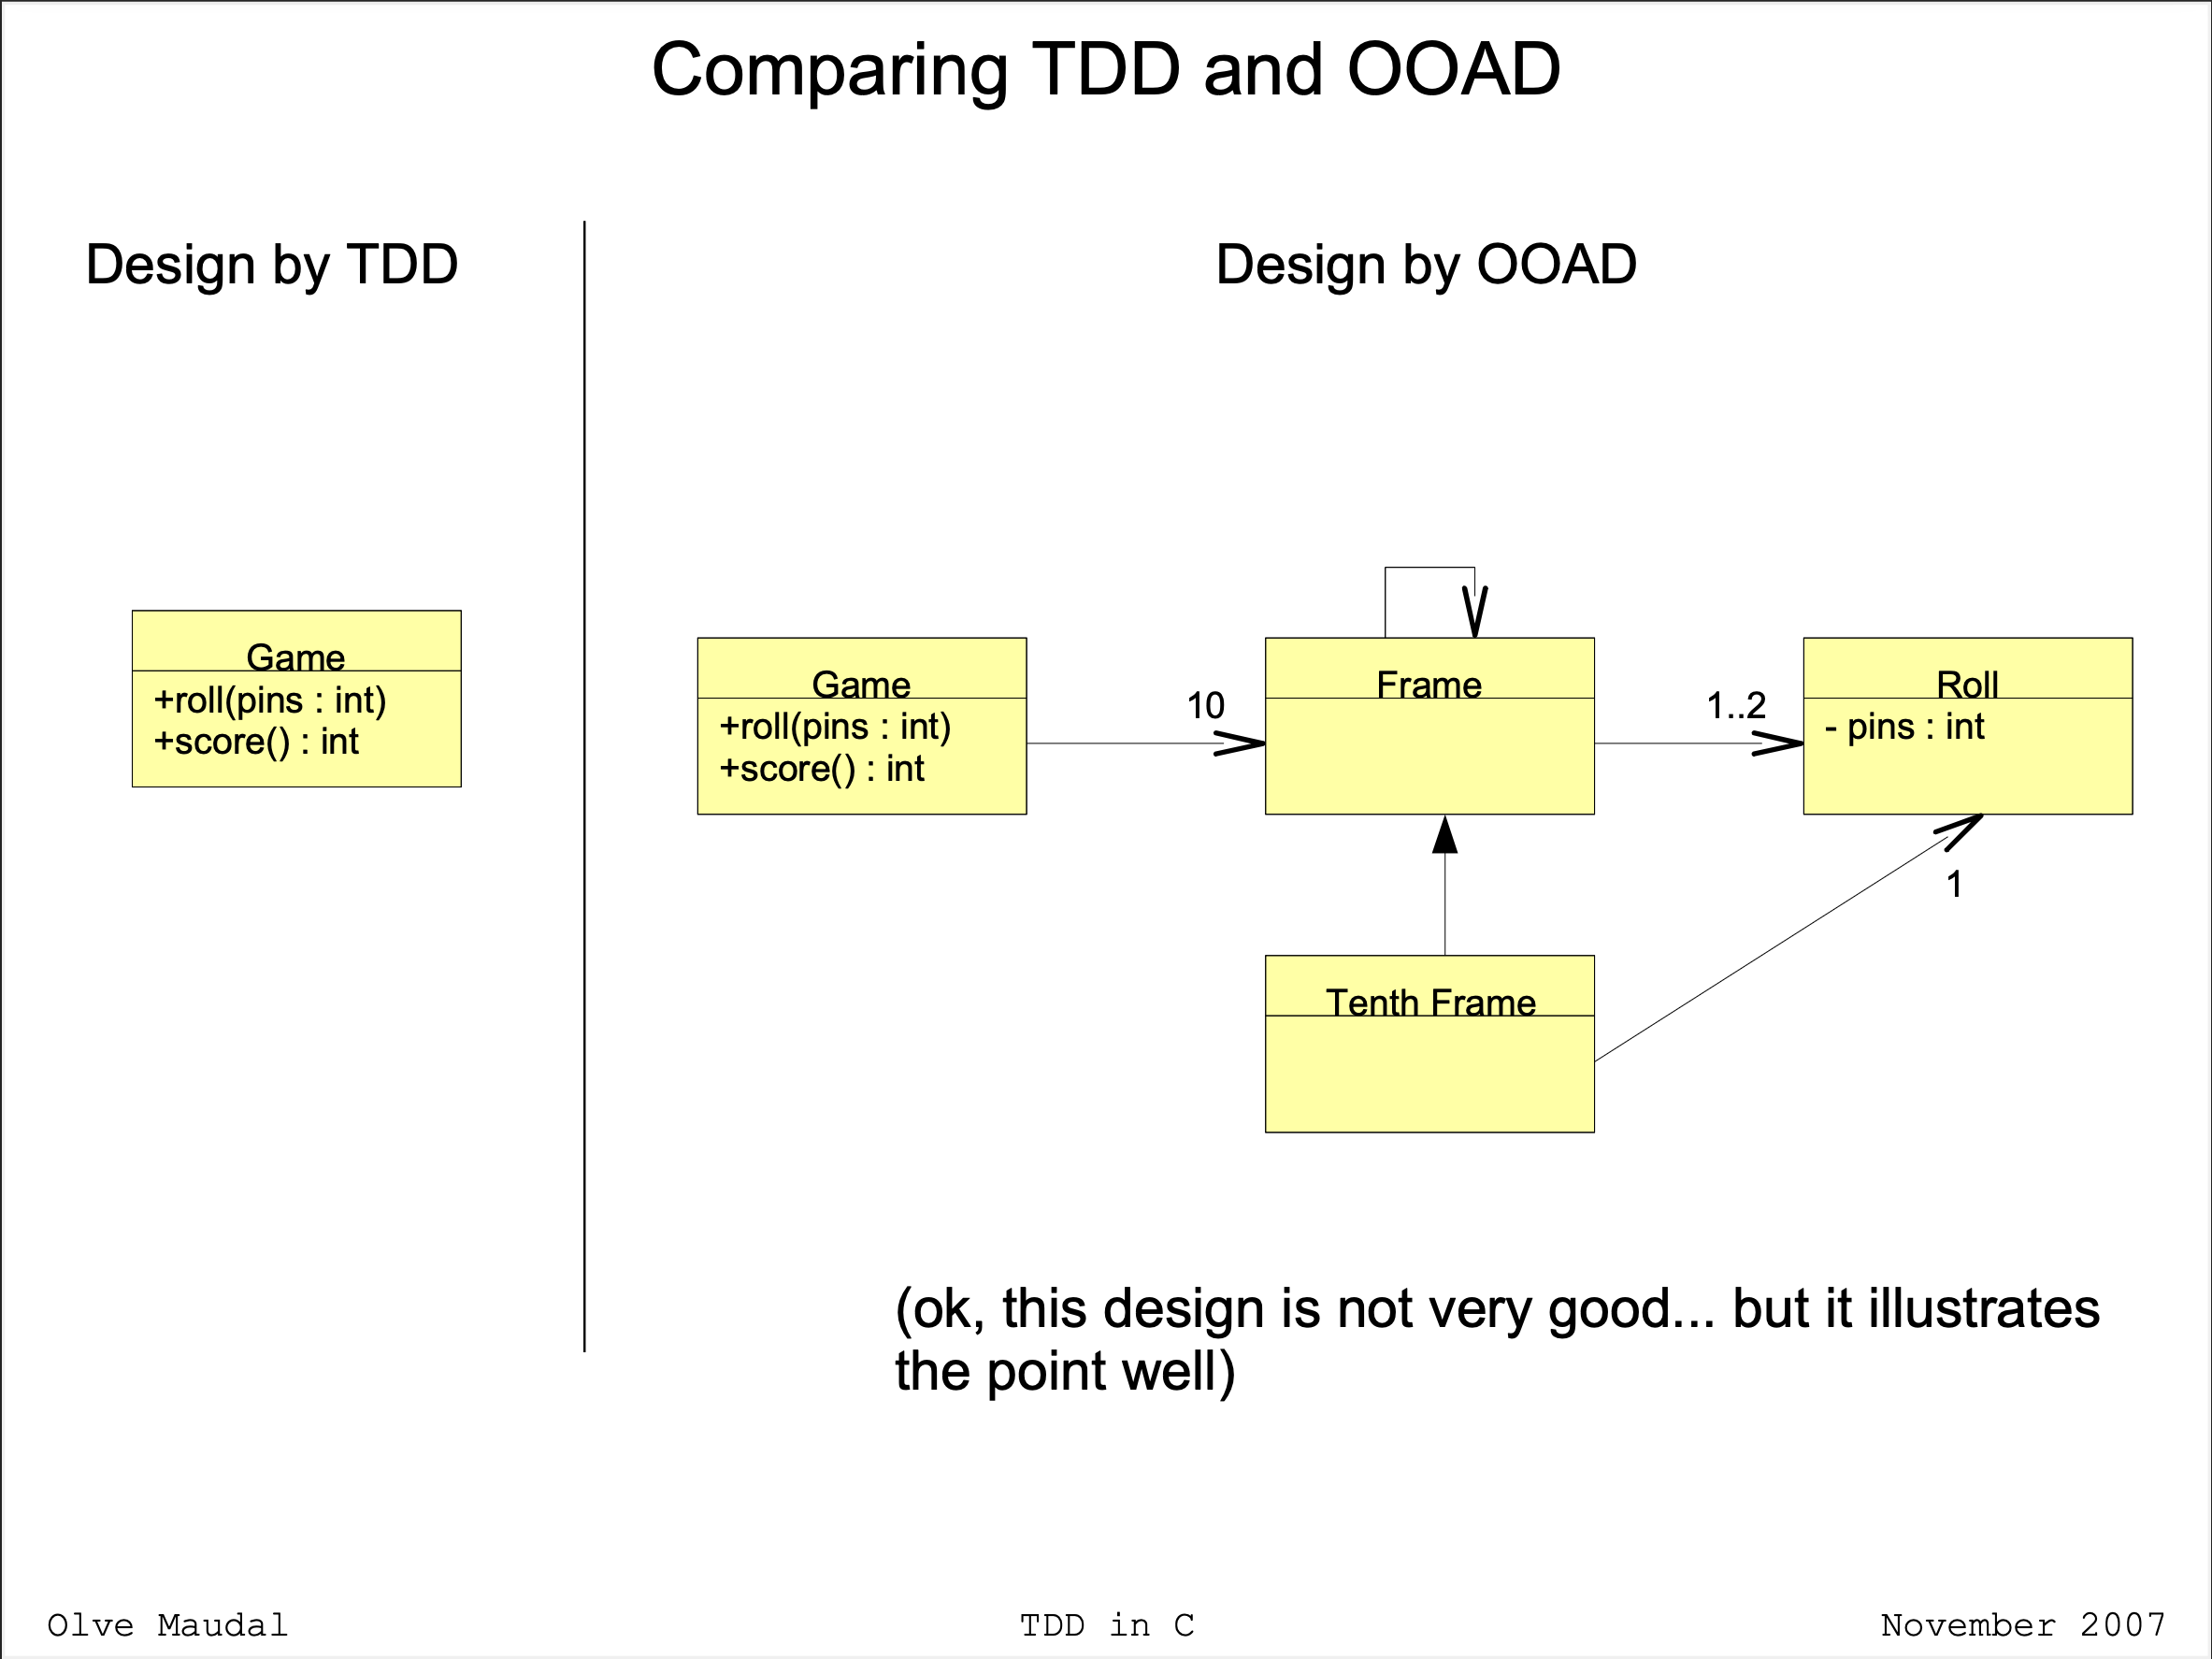
\includegraphics[width=\textwidth]{bowling-kata.png}
    \caption{\textit{Comparación entre el diseño del juego de
    los bolos a partir de implementación orientada a objetos
    y a partir de pruebas unitarias como se expone en \cite{TDD}.
    Diapositiva extraída de \cite{BowlingKata}.}}
\end{figure}

\subsubsection{¿Cuándo tiene sentido aplicar \textit{TDD}?}

Aunque muchas de las ideas del método \textit{TDD} son relevantes
y útiles a la hora de desarrollar cualquier pieza de software hay casos
en los que seguir el método es contraproducente.

Aunque las ideas del método son útiles y aplicables en otros ámbitos
tiene poco o ningún sentido aplicarlo rigurosamente en otros ámbitos o
en otros niveles; No deja de ser un método para modelar sistemas en
términos de módulos comprobados unitariamente.

\cite{TDD} expone la siguiente idea.
De poco sirve hacer un test que duplique la lógica que implementamos. Las
pruebas que debemos desarrollar a la hora de seguir el método tienen que
\textit{declarar} el funcionamiento, y hacerlo de una forma que permita que
este sea comprobable. De alguna forma, no se suele divulgar.

\subsubsection{\textit{TDD} como herramienta de modelado}

El 29 de agosto del 2023 escribo el siguiente hilo de mensajes en SWAD.

\begin{quote}
``\itshape{%
    Me hubiese gustado que Stroganoff hubiese sido menos vago en su exposición dado
    que la orientación a objetos da mucho más de lo que hablar.

    ¿Sabes qué? Un mes antes de empezar la carrera compré un ejemplar de segunda mano
    del «Programming: Principles and Practice Using C++». \cite{Stroganoff} Aprendí a
    programar en C++ a partir de ese libro. Una vez entendí cómo funcionan fundamentalmente
    los streams, librería estándar, posibles retornos de error y templates (entre otras
    muchas posibilidades divertidas del lenguaje), perdí el interés por la tecnología
    (el lenguaje) y, dado que la complejidad de mis programas eran inherentemente altos,
    en el segundo año de carrera empecé a interesarme por Plan9 \cite{Plan9} y el
    Código Limpio \cite{CleanCode} entre otros.

    Estas publicaciones junto a este libro despertaron otras inquietudes. A destacar,
    diseño de interfaces, «claridad» del código, planificación de desarrollo de software,
    etc. Paralelamente, al encontrar en las redes un sentimiento de aversión generalizado
    ante las metodologías ágiles, habiendo escuchado lo que Robert Cecil Martin opinaba
    acerca de las susodichas, decidí leerme el libro «Clean Agile: Back to Basics» \cite{AgileBackToBasics}.

    ¡Cuál fue mi sorpresa! ¡Al igual que ocurre con las Sagradas Escrituras, todo el mundo 
    habla de sus contenidos, pero nadie visita ni estudia los originales!

    Aprendí a escribir «código limpio». Apliqué gran parte de la convención de estilo.
    \textbf{Los problemas se transformaron}. Aun así seguí aplicándolo, puesto que
    prefería los problemas nuevos a los antiguos. Además, pertenecía a la selecta y
    superior élite de limpiadores de código, o esa sensación me causaba.

    Durante este tiempo intenté varias veces aprender TDD a través de Internet. Una
    experiencia bastante frustrante y hueca. Decidí estudiar «Test-Driven Development
    by Example» \cite{TDD}.

    «Al conocer esto, el estudiante alcanzó la iluminación».

    Empecé a sostener la siguiente tesis: \textbf{OOP funciona (más o menos) en tanto
    que obliga a definir interfaces}. No por añadir distracciones a los lenguajes las
    reglas que codificamos en software dejarán de ser inherentemente complejas.
    Sin embargo, una buena interfaz sí permitirá a nuestro cerebro saber qué se espera
    que nos tiene que devolver un servicio, y si nos lo está devolviendo correctamente.
    En muchas ocasiones, \textbf{TDD es una herramienta que ayuda a encontrar esas
    interfaces}.

    Hoy día escribo mis programas en C, la mayoría del tiempo sin necesitar reservar
    memoria dinámica más que en casos muy concretos en los que tenga que lidiar con
    ciertos servicios reentrantes o no sepa requerimientos en tiempo de compilación
    (en parte esto es gracias a los dominios con los que suelo trabajar). Dada una
    de mis muchas unidades de código, según voy escribiendo tests para esta, mi
    programa se simplifica y la interfaz se vuelve más clara.

    Cuando las reglas del juego cambian para mi cliente sé que tendré que ofrecerle
    una solución ante sus nuevos problemas. Sé que ocurrirán regresiones en cada nuevo
    lanzamiento. Compruebo cómo mis flujos de Integración Continua las detectan y las arreglo.

    Poco a poco la programación deja de tener mística, doctrina y emoción, y pasa a
    convertirse en algo mundano, tranquilo y aburrido.

    Comparto algunos recursos interesantes.

    \url{https://www.youtube.com/watch?v=tD5NrevFtbU}

    \url{https://www.youtube.com/@ContinuousDelivery/videos}

    \url{http://electronvector.com/how-to-use-ceedling-for-embedded-test-driven-development}

    \url{https://www.youtube.com/watch?v=xmiXmN6Rf3M}

    \url{http://www.catb.org/~esr/writings/unix-koans/}

    \url{https://web.mit.edu/~simsong/www/ugh.pdf}%
}''
\end{quote}

\section{Estimación de costes}

La estimación de costes en los proyectos informáticos suelen
ser significativamente erróneos. Nosotros nos apoyamos en dos
recursos que han probado ser veraces para nuestras estimaciones.

\begin{enumerate}
    \item \textbf{Desglose}. Cuanto más desglosemos lo que
          necesita una tarea para llevarse a cabo con más
          certeza podremos especificar tanto costes materiales
          como temporales.
    \item \textbf{Datos pasados}. Como registramos, categorizamos
          y describimos todo el tiempo que dedicamos al trabajo
          registrando fecha en la que se efectúa el trabajo, hora
          de inicio y hora de fin podemos muchas veces inferir
          cuánto tiempo hará falta para cada una de las actividades
          del desglose.
\end{enumerate}

Dentro de esta estimación también tenemos en cuenta los costes de
oportunidad (¿si en vez de hacer este proyecto, hiciese este otro,
ganaría más? ¿si no lo hago, perdería?) y los costes de soporte del proyecto.

\section{Seguimiento del desarrollo por parte del cliente}

Gracias a que el cliente puede conocer en cualquier momento a qué 
parte del proyecto nos estamos dedicando puede darse cuenta,
gracias a la información que posee, de que estemos dedicando tiempo
o esfuerzo a un aspecto del proyecto que él no considere tan
relevante. También puede planificar apartar una máquina para poder
testar un hito en el desarrollo del proyecto en la máquina objetivo.

Usamos un documento que nos sirve de guía en nuestro trabajo, y que
vamos actualizando según vamos implementando características.
Compartimos este documento con el cliente periódicamente.
Llamamos a este documento \textbf{Plan de desarrollo}.

Cada vez que liberamos una versión compartimos otro documento llamado
\textit{\textbf{Changelog}}\footnote{Histórico de cambios.}. Escribimos
este documento a partir de las descripciones de las contribuciones al
repositorio.

\section{Seguimiento del coste y tiempo dedicado al proyecto}

Para poder facturar por nuestros servicios, y para realizar estimaciones
basadas en datos, registramos los gastos asociados al proyecto.

Cuando compramos algo registramos su fecha de compra, precio y función.

Cuando trabajamos:
\begin{enumerate}
    \item Categorizamos nuestro trabajo. ¿Estamos organizando la producción?
          ¿Programando? ¿Haciendo un desglose de componentes? ¿Dando soporte
          telefónico? etc.
    \item Registramos la fecha en que lo hacemos. Registramos la hora de inicio
          y la hora de fin.
    \item Registramos un comentario claro y conciso acerca de qué hemos hecho.
\end{enumerate}

\subsection{¿Por qué facturar por horas y no por servicio?}

Dentro de mi precio por hora están incluidos otros gastos muy relevantes como son:

\begin{enumerate}
    \item Cuota de la Seguridad Social.
    \item Retenciones del Impuesto sobre la Renta de las Personas Físicas.
    \item Coste amortizado de equipamiento para llevar a cabo la actividad.
    \item Dietas.
\end{enumerate}

Yo, como trabajador autónomo, ofrezco servicios a mi empresa a precio de mercado\footnote{%
    ¿Cuánto gana de media \textbf{después de impuestos} un empleado que realizase mis mismas
    funciones, tuviese la misma disponibilidad, las mismas responsabilidades, con mis años
    de experiencia, con mis conocimientos y en mi sector?
}
sumándole a mayores estos gastos.

Es la empresa la que cobra a mi cliente por servicio.

En caso de acabar el año con superávit reinvertimos en la empresa.
